\section{Vulnerability: Tokens are 1-10 and don't expire}
\label{sec:background}
\textbf{Description:} The access tokens on the website have 2 key issues. Firstly there are only ten eleven tokens availabe (0 through to 10). Secondly the tokens have no expiry
date and as such if a hacker were to gain access to a token through for example Javascript injection as seen in vulnerability 3, he could use it to keep permanent access to a
user's account even if they changed their password, regardless of how complex the password hashing was made. This of course is a serious security flaw and needs to be addressed.
By only having 11 tokens this flaw is made worse since an attacker would only need to try 11 tokens in order to get access. \\ \\
\textbf{Testing the Vulnerability:} To do this I logged in as \textit{hacker@wondoughbank.com} and displayed the transactions. After my fix to the login issue in the previous
vulnerability the result was identical to figure \ref{figvun6}. I then went into the developer options on my browser to display the cookies:
\begin{figure}[h]
    \centering
    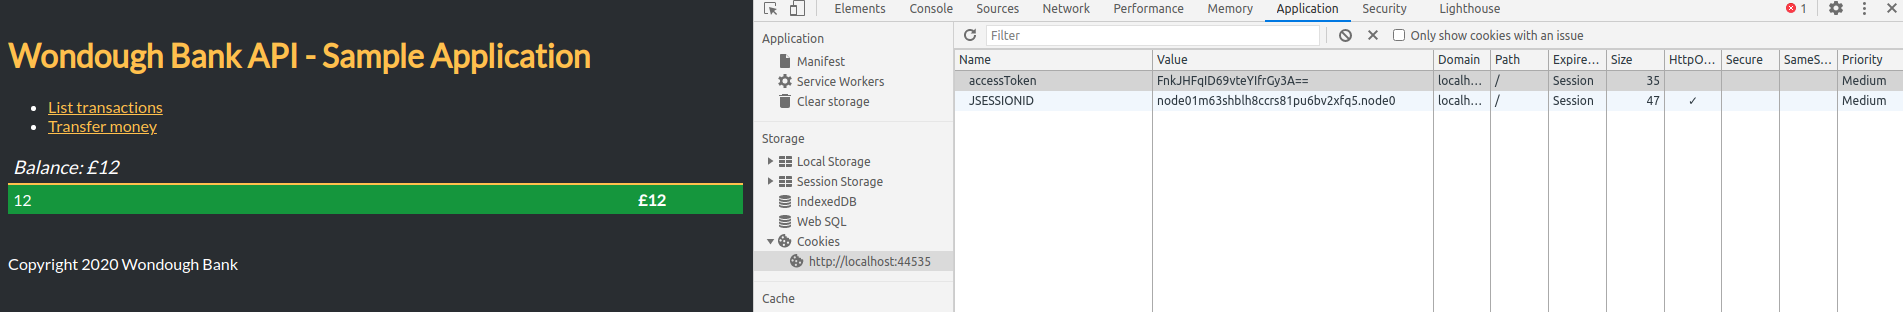
\includegraphics[width=1\textwidth]{figs/7.1.png}
    \caption{The token visible in the cookies of my session}
    \label{7.1}
\end{figure}\\
From here I was able to change the token to one associated with user 0 (from \textit{jxTkX87qFnpaNt7dS+olQw==} to \textit{jxTkX87qFnpaNt7dS+olQw==})
\begin{figure}[h]
    \centering
    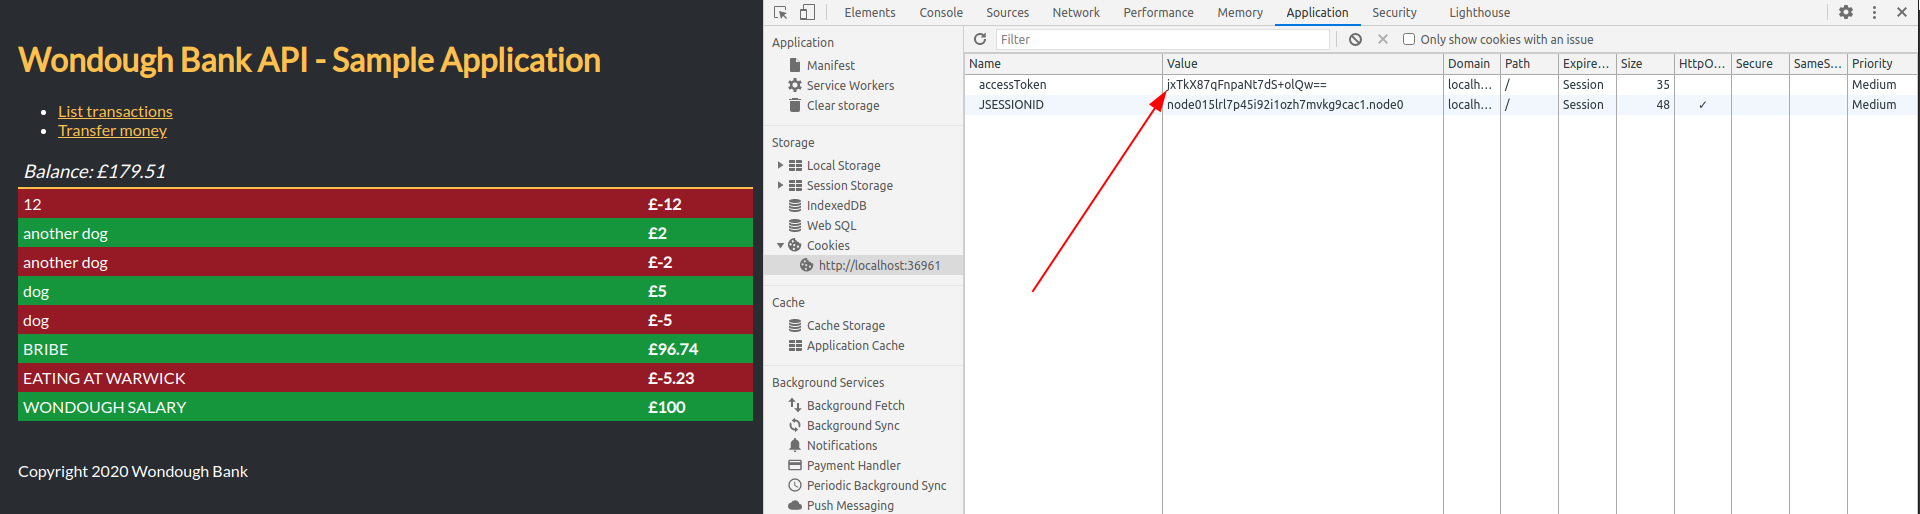
\includegraphics[width=1\textwidth]{figs/7.2.png}
    \caption{By editing the token I gain access to the intern's account}
    \label{7.2}
\end{figure}\\
\textbf{Mitigation:} The first issue of the 0-10 occurs in \verb|dbConnection| where the following code is used to create the tokens id:\\
\begin{minted}{java}
app.setRequestToken(Integer.toString(this.largestRequestToken(), 10));
app.setAccessToken(Integer.toString(this.largestAccessToken(), 10));
\end{minted}
I have therefore chosen to use the salt generation as the token since this is unique each time and much more complex. It also means that the issue of the access and request token
being the same solved.
\begin{minted}{java}
String salt;
salt = Program.getInstance().getSecurityConfiguration().generateSalt();
app.setRequestToken(salt);
salt = Program.getInstance().getSecurityConfiguration().generateSalt();
app.setAccessToken(salt);
\end{minted}
Since the salt is random each time this allows us to solve the issue of recurring tokens. To solve the issue of the fact the tokens never expire an additional column was added to
the database called \verb|expiryDate|, which was a \verb|TimeStamp| and represented the point in time when that key would no longer be valid. To set this I edited the
\verb|createApp()| function in \verb|dbConnection|. A fourth value was added to the prepared statement, which is a TimeStamp. From there the current time is stored and 30 minutes
added to it. This is to be the value of the \verb|expiryDate| of the access token. Whilst the request token has a date of 1 hour from now. The choice of times was to ensure the security
of the website was as rigorous as possible. This choice of time meant there's time to generate new access and request tokens after the access token is expired.
The request tokens will expire a little while later and can get purged in a timely manner to avoid accumulation \cite{tokens}. It also means if a hacker were to gain access to a token
it would expire shortly making access limited. However inorder to give the keys different expiry times they had to be stored seperatly, as such the function was altered to create
two entries into the database, one with request token as null and one with access token as null.
\begin{figure}[h]
    \centering
    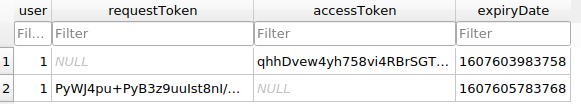
\includegraphics[width=1\textwidth]{figs/token2.png}
    \caption{The adapted way of storing tokens}
    \label{7.2}
\end{figure}\\
The expiry times were set as follows:
\begin{minted}{java}
Timestamp now;
now = new Timestamp(System.currentTimeMillis());
now.setTime(now.getTime() + TimeUnit.MINUTES.toMillis(30));
stmt.setTimestamp(4, now);

now = new Timestamp(System.currentTimeMillis());
now.setTime(now.getTime() + TimeUnit.HOURS.toMillis(1));
stmt.setTimestamp(4, now);
\end{minted}
Finally a remove tokens function was created that would be called regularly to remove outdated tokens. It checked if the expiry date of the token had been surpassed by comparing
it to the current time:
\begin{minted}{java}
long ut1 = System.currentTimeMillis();
String query3 = "DELETE FROM authorised_apps "
                +"WHERE expiryDate < "+ ut1 + ";";
Statement stmt2 = this.connection.createStatement();
int rs = stmt2.executeUpdate(query3);
\end{minted}
From this an automatic test was devised to ensure all these new criteria were met. It would create temporary tokens, ensure the difference in expiration date, value and then check
they would be removed in an hours time. The randomness and greater complecity of the tokens alongside their limited time means this vulnerability has been mitigated as far as 
possible.

